\documentclass{beamer}
\usetheme{Madrid}
\usecolortheme{default}

\usepackage[utf8]{inputenc}
\usepackage{amsmath,amssymb}   % math symbols
% \usepackage{bm}                 % bold math vectors
\usepackage{xcolor}             % colors
\usepackage{graphicx}           % images
\usepackage{listings}           % code listing
\usepackage{courier}    % monospace font for code
\usepackage{gvv}

% Optional: customize Python highlighting in listings
\lstset{
    language=Python,
    basicstyle=\ttfamily\small,       % font and size
    keywordstyle=\color{blue},
    stringstyle=\color{orange},
    commentstyle=\color{green!60!black},
    showstringspaces=false,
    breaklines=true,
    numbers=left,
    numberstyle=\tiny\color{gray},
    frame=single,                     % frame around code
    tabsize=4
}

\lstset{
    language=C,
    basicstyle=\ttfamily\small,
    keywordstyle=\color{blue},
    stringstyle=\color{orange},
    commentstyle=\color{green!60!black},
    numbers=left,
    numberstyle=\tiny\color{gray},
    breaklines=true,
    showstringspaces=false,
}


\title{4.13.36}
\author{Sai Sreevallabh - EE25BTECH11031}
\date{October 4, 2025}

\begin{document}

\frame{\titlepage}

\begin{frame}{Question}
Let $PQR$ be a right angled isosceles triangle, right at $P(2, 1)$. If the equation of the line $QR$ is $2x + y = 3$, then the equation representing the pair of lines $PQ$ and $PR$ is \\

\begin{enumerate}
        \item $3x^2 - 3y^2 + 8xy + 20x + 10y + 25 = 0$
        \item $3x^2 - 3y^2 + 8xy - 20x - 10y + 25 = 0$
        \item $3x^2 - 3y^2 + 8xy + 10x + 15y + 20 = 0$
        \item $3x^2 - 3y^2 - 8xy - 10x - 15y - 20 = 0$
\end{enumerate}

\end{frame}

\begin{frame}{Theoretical Solution}

Given point is $\vec{P} = \myvec{2\\1}$ and given line can be written as 
\begin{align}
    \vec{n}^\top\vec{x} = c \label{eq1}
\end{align}

where, $\vec{n} = \myvec{2\\1}$ and $c = 3$.\\

Parametric form of line through $\vec{P}$ is 
\begin{align}
    \vec{r} = \vec{P} + \lambda\vec{m}
\end{align}

\end{frame}

\begin{frame}{Theoretical Solution}

Using this, we can represent points $Q$ and $R$ as
\begin{align}
    \vec{Q} = \vec{P} + \lambda_1\vec{m_1}\label{eq3}
\end{align}

\begin{align}
    \vec{R} = \vec{P} + \lambda_2\vec{m_2} \label{eq4}
\end{align}

where, $\vec{m_1} = \myvec{1\\m_1}$ and $\vec{m_2} = \myvec{1\\m_2}$ are direction vectors of lines $\vec{Q-P}$ and $\vec{R-P}$, while $m_1$ and $m_2$ are the respective slopes.\\

\end{frame}

\begin{frame}{Theoretical Solution}
Given that the lines are perpendicular, 
\begin{align}
    \vec{m_1}^\top\vec{m_2} =& 0\\
    \implies m_1m_2 =& -1
\end{align}

Substituting equation \eqref{eq3} in \eqref{eq1}
\begin{align}
    \vec{n}^\top\brak{\vec{P} + \lambda_1\vec{m_1}} = c\\
    \implies \lambda_1 \ = \ \frac{c-\vec{n}^\top\vec{P}}{\vec{n}^\top\vec{m_1}}
\end{align}

\end{frame}

\begin{frame}{Theoretical Solution}
Substituting the values, we get
\begin{align}
    \lambda_1 \ = \ \frac{-2}{2+m_1} \label{eq9}
\end{align}

Similarly, substituting equation \eqref{eq4} in \eqref{eq1}
\begin{align}
    \lambda_2 \ = \ \frac{c-\vec{n}^\top\vec{P}}{\vec{n}^\top\vec{m_2}}
\end{align}

Substituting values,
\begin{align}
    \lambda_2 \ =&\ \frac{-2}{2+m_2}\\
    \implies \lambda_2 \ =& \ \frac{-2m_1}{2m_1-1} \label{eq12}
\end{align}\\
\end{frame}

\begin{frame}{Theoretical Solution}
Let $\vec{M}$ be the midpoint of $\vec{Q-R}$:
\begin{align}
    \vec{M} = \frac{\vec{Q+R}}{2}
\end{align}

Since $\triangle PQR$ is isosceles,
\begin{align}
    \vec{P}-\vec{M} \perp \vec{Q}-\vec{R}\\
    \implies \brak{\vec{P}-\frac{\vec{Q+R}}{2}}^\top \brak{\vec{Q}-\vec{R}} = 0
\end{align}\\
\end{frame}

\begin{frame}{Theoretical Solution}
    Substituting values from \eqref{eq3}, \eqref{eq4}, we get
\begin{align}
    \brak{\lambda_1\vec{m_1}+\lambda_2\vec{m_2}}^\top\brak{\lambda_1\vec{m_1}-\lambda_2\vec{m_2}} =& 0\\
    \lambda_1^2\vec{m_1}^\top\vec{m_1} =& \lambda_2\vec{m_2}^\top\vec{m_2}\\
    \lambda_1^2\brak{1+m_1^2} =& \lambda_2\brak{1+\frac{1}{m_1^2}}\\
    \abs{\lambda_1}=& \abs{\frac{\lambda_2}{m_1}}
\end{align}\\

Substituting values of $\lambda_1$ and $\lambda_2$ from \eqref{eq9} and \eqref{eq12}

\begin{align}
    \abs{ \frac{2}{2+m_1}} =& \abs{\frac{2}{2m_1-1}}
\end{align}
\end{frame}

\begin{frame}{Theoretical Solution}

Solving the above, we get
\begin{align}
    m_1 = 3 \ \text{or} \ m_1 = \frac{-1}{3}
\end{align}

Correspondingly,
\begin{align}
    m_2 = \frac{-1}{3} \ \text{or} \ m_2 = 3
\end{align}\\

So, the equations of the two required lines are
\begin{align}
    3x-y-5=0 \ \ \text{and}\ \ x+3y-5=0
\end{align}\\

$\therefore$ Multiplying the above two equations, we get the pair of straight lines to be 
\begin{center}
   $3x^2 - 3y^2 + 8xy - 20x - 10y + 25 = 0$
\end{center} 
\end{frame}

\begin{frame}[fragile]
    \frametitle{C Code - Solving Using Gaussian Elimination}

    \begin{lstlisting}
#include <stdio.h>

void Solve_Gaussian(double A[3], double B[3], double sol[2]) {
    // If A[0] == 0, swap rows to avoid division by zero
    //Also covers the case where the matrix is diagonal.
    if (A[0] == 0) {
        for (int i = 0; i < 3; i++) {
            double temp = A[i];
            A[i] = B[i];
            B[i] = temp;
        }
    }

    \end{lstlisting}

\end{frame}

\begin{frame}[fragile]
    \frametitle{C Code - Solving Using Gaussian Elimination}

    \begin{lstlisting}
    
    double factor = B[0] / A[0];
    for (int i = 0; i < 3; i++) {
        B[i] = B[i] - factor * A[i];
    }

    sol[1] = B[2] / B[1];
    sol[0] = (A[2] - A[1] * sol[1]) / A[0];
}

    \end{lstlisting}

\end{frame}

\begin{frame}[fragile]
    \frametitle{Python Code - Using Shared Object}
    \begin{lstlisting}
import ctypes
import numpy as np
import matplotlib.pyplot as plt

c_lib = ctypes.CDLL("./code.so")

c_lib.Solve_Gaussian.argtypes = [ctypes.c_double*3, ctypes.c_double*3, ctypes.c_double*2]

#line QR
A = (ctypes.c_double*3)(2,1,3)

#line PR
B = (ctypes.c_double*3)(3,-1,5)

#line PQ
C = (ctypes.c_double*3)(1,3,5)



\end{lstlisting}
\end{frame}

\begin{frame}[fragile]
    \frametitle{Python Code - Using Shared Object}
    \begin{lstlisting}

P = np.array([2,1])

Q = (ctypes.c_double*2)(0.0,0.0)
c_lib.Solve_Gaussian(A,C,Q)

R = (ctypes.c_double*2)(0.0,0.0)
c_lib.Solve_Gaussian(A,B,R)

plt.scatter([P[0],Q[0],R[0]], [P[1],Q[1],R[1]])

plt.plot([P[0],R[0]],[P[1],R[1]], label = "PR: 3x-y=5")
plt.plot([P[0],Q[0]],[P[1],Q[1]], label = "PQ: x+3y=5")
plt.plot([0,2], [3,-1], c='green', label = "QR: $2x+y=3$")

\end{lstlisting}
\end{frame}

\begin{frame}[fragile]
    \frametitle{Python Code - Using Shared Object}
    \begin{lstlisting}
    
R_p = np.array([R[0],R[1]], dtype=np.float64).reshape(-1,1)
Q_p = np.array([Q[0],Q[1]], dtype=np.float64).reshape(-1,1)
P_p = np.array([2,1]).reshape(-1,1)


tri_coords = np.block([[P_p,Q_p,R_p]])
plt.scatter(tri_coords[0,:], tri_coords[1,:])
vert_labels = ['P','Q','R']
for i, txt in enumerate(vert_labels):
    plt.annotate(f'{txt}\n',
                 (tri_coords[0,i], tri_coords[1,i]), 
                 textcoords="offset points", 
                 xytext=(0.2,0.2), 
                 ha='center') 

\end{lstlisting}
\end{frame}

\begin{frame}[fragile]
    \frametitle{Python Code - Using Shared Object}
    \begin{lstlisting}
    
ax = plt.gca()
ax.spines['top'].set_color('none')
ax.spines['bottom'].set_position('zero')
ax.spines['right'].set_color('none')
ax.spines['left'].set_position('zero')
plt.xlabel('x')
plt.ylabel('y')
plt.legend(loc='best')
plt.grid()
plt.axis('equal')

plt.savefig("../Figs/plot(py+C).png")
plt.show()



\end{lstlisting}
\end{frame}

\begin{frame}{Plot-Using Both C and Python}
    \centering
    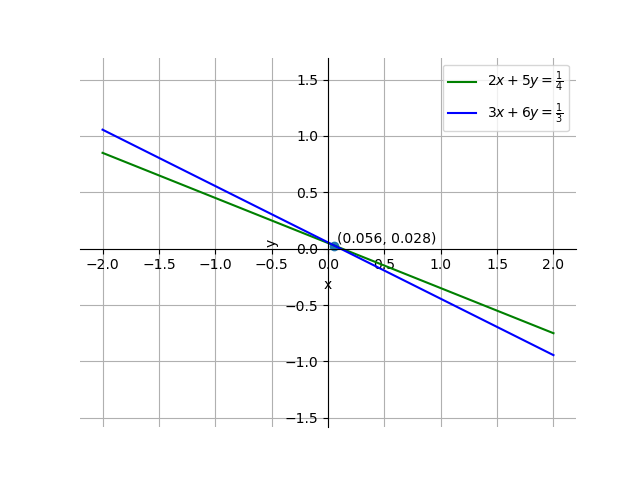
\includegraphics[width=\columnwidth, height=0.8\textheight, keepaspectratio]{Figs/plot(py+C).png}     
\end{frame}

%-------End of Python+C-------------


\begin{frame}[fragile]
    \frametitle{Python Code}
    \begin{lstlisting}

import numpy as np
import matplotlib.pyplot as plt
import numpy.linalg as LA

P = np.array([2, 1])

#solving Ax=b, to find x
A = np.array([[3, -1],
              [2,  1]])
b = np.array([5, 3])
R = LA.solve(A, b)

A = np.array([[1, 3],
              [2, 1]])
b = np.array([5, 3])
Q = LA.solve(A, b)



\end{lstlisting}
\end{frame}

\begin{frame}[fragile]
    \frametitle{Python Code}
    \begin{lstlisting}
plt.scatter([P[0],Q[0],R[0]], [P[1],Q[1],R[1]])

plt.plot([P[0],R[0]],[P[1],R[1]], label = "PR: 3x-y=5")
plt.plot([P[0],Q[0]],[P[1],Q[1]], label = "PQ: x+3y=5")
plt.plot([0,2], [3,-1], c='green', label = "QR: $2x+y=3$")

R_p = np.array([R[0],R[1]], dtype=np.float64).reshape(-1,1)
Q_p = np.array([Q[0],Q[1]], dtype=np.float64).reshape(-1,1)
P_p = np.array([2,1]).reshape(-1,1)


\end{lstlisting}
\end{frame}

\begin{frame}[fragile]
    \frametitle{Python Code}
    \begin{lstlisting}

tri_coords = np.block([[P_p,Q_p,R_p]])
plt.scatter(tri_coords[0,:], tri_coords[1,:])
vert_labels = ['P','Q','R']
for i, txt in enumerate(vert_labels):
    plt.annotate(f'{txt}\n',
                 (tri_coords[0,i], tri_coords[1,i]), 
                 textcoords="offset points", 
                 xytext=(0.2,0.2), 
                 ha='center') 


\end{lstlisting}
\end{frame}

\begin{frame}[fragile]
    \frametitle{Python Code}
    \begin{lstlisting}

ax = plt.gca()
ax.spines['top'].set_color('none')
ax.spines['bottom'].set_position('zero')
ax.spines['right'].set_color('none')
ax.spines['left'].set_position('zero')
plt.xlabel('x')
plt.ylabel('y')
plt.legend(loc='best')
plt.grid()
plt.axis('equal')

plt.savefig("../Figs/plot(py).png")
plt.show()

\end{lstlisting}
\end{frame}


\begin{frame}{Plot-Using Python only}
    \centering
    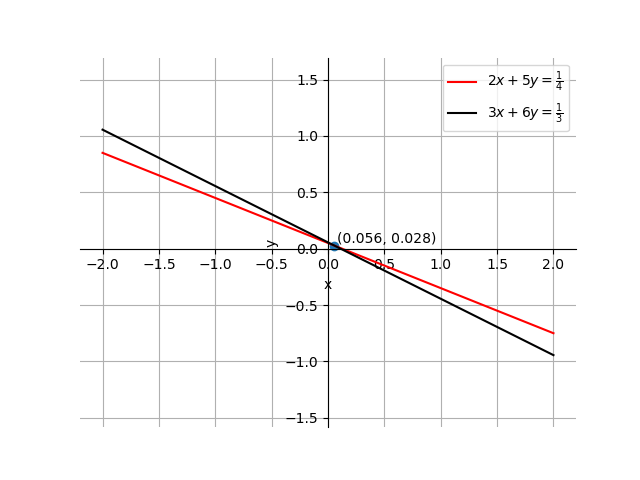
\includegraphics[width=\columnwidth, height=0.8\textheight, keepaspectratio]{Figs/plot(py).png}     
\end{frame}


\end{document}

